\documentclass[twocolumn]{revtex4}
\usepackage{graphics,graphicx,epsfig,ulem,amsmath,multirow,gensymb,commath,textcomp}
\newcommand{\squeezeup}{\vspace{-2.5mm}}

\begin{document}

\textheight=26.385cm
%Change textheight as the last resort...

\title{Optical Fourier Transforms}
 
\author{Jacky Cao, Room 205, Friday, Lab Partners: Thomas Spriggs \\ Date of experiment: 10/02/2017 to , Date of report: 20/11/2016}

\begin{abstract}              
Through the study of the Fourier Transforms of blah blah blah. \cite{crc}. 
\end{abstract}

\maketitle

\section{Introduction} 
\vspace{-2ex} 

Intro

\begin{equation}
35000 \times [\frac{sin[\frac{1}{47} \times (x-690)]}{\frac{1}{47} \times (x-690)}]^2
\end{equation}

\vspace{-3ex}
\section{Method} 
\vspace{-2ex}

Method

\begin{figure}[!h]
\begin{center}
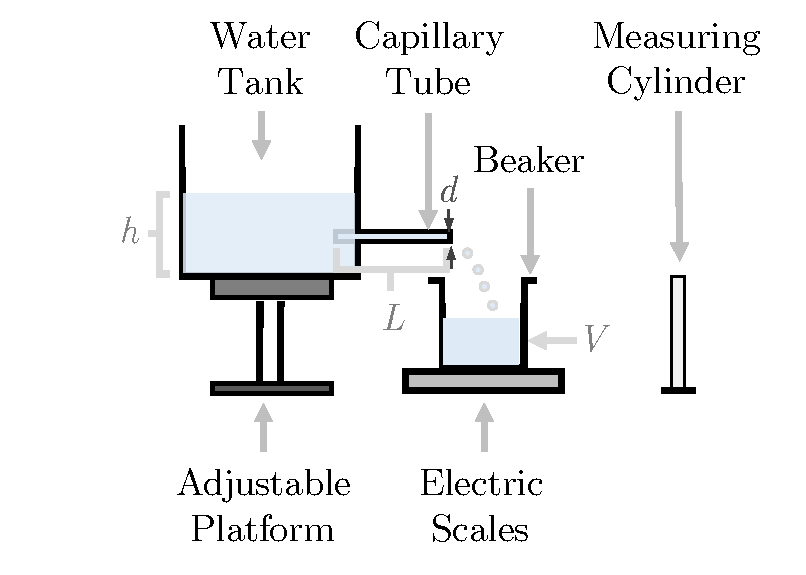
\includegraphics[width=5.7cm]{fig1}
\caption[]{A schematic of the experimental set-up used to collect data. }
\label{fig:fig1}
\end{center}
\end{figure}

Method

\vspace{-3ex}
\section{Results}
\vspace{-2ex}

Results

\begin{table}[h!]
\centering
\begin{tabular}{c@{\hskip 20pt}c@{\hskip 20pt}c@{\hskip 20pt}c} 
 \hline
 \textbf{Tube} & \textbf{Radius, a [mm]} & \textbf{$\boldsymbol{\eta}$ [mPa {s}]} & \textbf{$\boldsymbol{\chi^2_{\nu}}$} \\ [0.5ex] 
 $Blue$ &$0.55\pm0.03$ & $1.0\pm0.2$ & 11.0 \\ 
 $Red$ & $0.47\pm0.03$ & $1.1\pm0.3$ & 5.31 \\
 $Black$ & $0.46\pm0.03$ & $1.0\pm0.3$ & 1.94 \\
 
 \hline
\end{tabular}
\caption{For each tube is shown its radius, their respective calculated value for the viscosity of water $\eta$, and the reduced chi-squared statistic, $\chi^2_{\nu}$.}
\label{table:1}
\end{table}

\vspace{-3ex}
\section{Discussion}
\vspace{-2ex}

Discussion

\vspace{-5ex}
\section{Conclusions}
\vspace{-2ex}

Conclusion

\begin{thebibliography}{5}
\bibitem{poiseuillehagen}
	Salvatore P. Sutera and Richard Skalak
	\textit{The History of Poiseuille's Law}.
	Annu. Rev. Fluid Mech., 1993.
	
\bibitem{collegephysics}
	Raymond A. Serway, Chris Vuille, and Jerry S. Faughin
	\textit{College Physics, 8th Edition}.
	Brooks/Cole, Belmont, CA, USA, 2009.

\bibitem{youngandfreedman} 
	Hugh D. Young and Roger A. Freedman.
	\textit{University Physics with Modern Physics, 13th Edition}. 
	Pearson Education Limited, Essex, UK, 2015.
	
\bibitem{crc} 
	W. M. Haynes.
	\textit{CRC Handbook of Chemistry and Physics, 92nd Edition}. 
	CRC Press, Florida, USA, 2011.
	
\bibitem{dentemp} 
	J. L. Martin and S. C. McCutcheon
	\textit{Hydrodynamics and Transport for Water Quality Modelling}. 
	CRC Press, Florida, USA, 1999.
	
\bibitem{hughesandhayes} 
	I. G. Hughes and T. P. A. Hase
	\textit{Measurements and their Uncertainties}. 
	Oxford University Press, Oxford, UK, 2010.
	
\end{thebibliography}
\clearpage

\vfill
\twocolumngrid
\vspace{-3ex}
\section*{Appendix}
\vspace{-2ex}

Appendix


\clearpage
\end{document}